\documentclass[11pt,]{article}
\usepackage[left=1in,top=1in,right=1in,bottom=1in]{geometry}
\newcommand*{\authorfont}{\fontfamily{phv}\selectfont}
\usepackage[]{mathpazo}


  \usepackage[T1]{fontenc}
  \usepackage[utf8]{inputenc}




\usepackage{abstract}
\renewcommand{\abstractname}{}    % clear the title
\renewcommand{\absnamepos}{empty} % originally center

\renewenvironment{abstract}
 {{%
    \setlength{\leftmargin}{0mm}
    \setlength{\rightmargin}{\leftmargin}%
  }%
  \relax}
 {\endlist}

\makeatletter
\def\@maketitle{%
  \newpage
%  \null
%  \vskip 2em%
%  \begin{center}%
  \let \footnote \thanks
    {\fontsize{18}{20}\selectfont\raggedright  \setlength{\parindent}{0pt} \@title \par}%
}
%\fi
\makeatother




\setcounter{secnumdepth}{0}

\usepackage{longtable,booktabs}

\usepackage{graphicx,grffile}
\makeatletter
\def\maxwidth{\ifdim\Gin@nat@width>\linewidth\linewidth\else\Gin@nat@width\fi}
\def\maxheight{\ifdim\Gin@nat@height>\textheight\textheight\else\Gin@nat@height\fi}
\makeatother
% Scale images if necessary, so that they will not overflow the page
% margins by default, and it is still possible to overwrite the defaults
% using explicit options in \includegraphics[width, height, ...]{}
\setkeys{Gin}{width=\maxwidth,height=\maxheight,keepaspectratio}


\title{Additive influence of human-wildlife conflict and introduced mammalian
predation on the population dynamics of Kea (\emph{Nestor notabilis})  }



\author{\Large E.M. Kennedy\vspace{0.05in} \newline\normalsize\emph{Toi-Ohomai Institute of Technology}   \and \Large G.L.W. Perry\vspace{0.05in} \newline\normalsize\emph{University of Auckland}   \and \Large C.E. Simpkins\vspace{0.05in} \newline\normalsize\emph{University of Göttingen, University of Auckland}  }


\date{}

\usepackage{titlesec}

\titleformat*{\section}{\normalsize\bfseries}
\titleformat*{\subsection}{\normalsize\itshape}
\titleformat*{\subsubsection}{\normalsize\itshape}
\titleformat*{\paragraph}{\normalsize\itshape}
\titleformat*{\subparagraph}{\normalsize\itshape}


\usepackage{natbib}
\bibliographystyle{apsr}
\usepackage[strings]{underscore} % protect underscores in most circumstances



\newtheorem{hypothesis}{Hypothesis}
\usepackage{setspace}


% set default figure placement to htbp
\makeatletter
\def\fps@figure{htbp}
\makeatother


% move the hyperref stuff down here, after header-includes, to allow for - \usepackage{hyperref}

\makeatletter
\@ifpackageloaded{hyperref}{}{%
\ifxetex
  \PassOptionsToPackage{hyphens}{url}\usepackage[setpagesize=false, % page size defined by xetex
              unicode=false, % unicode breaks when used with xetex
              xetex]{hyperref}
\else
  \PassOptionsToPackage{hyphens}{url}\usepackage[draft,unicode=true]{hyperref}
\fi
}

\@ifpackageloaded{color}{
    \PassOptionsToPackage{usenames,dvipsnames}{color}
}{%
    \usepackage[usenames,dvipsnames]{color}
}
\makeatother
\hypersetup{breaklinks=true,
            bookmarks=true,
            pdfauthor={E.M. Kennedy (Toi-Ohomai Institute of Technology) and G.L.W. Perry (University of Auckland) and C.E. Simpkins (University of Göttingen, University of Auckland)},
             pdfkeywords = {conservation; extinction; human-induced mortality; population viability
analysis; population dynamics},  
            pdftitle={Additive influence of human-wildlife conflict and introduced mammalian
predation on the population dynamics of Kea (\emph{Nestor notabilis})},
            colorlinks=true,
            citecolor=blue,
            urlcolor=blue,
            linkcolor=magenta,
            pdfborder={0 0 0}}
\urlstyle{same}  % don't use monospace font for urls

% Add an option for endnotes. -----


% add tightlist ----------
\providecommand{\tightlist}{%
\setlength{\itemsep}{0pt}\setlength{\parskip}{0pt}}

% add some other packages ----------

% \usepackage{multicol}
% This should regulate where figures float
% See: https://tex.stackexchange.com/questions/2275/keeping-tables-figures-close-to-where-they-are-mentioned
\usepackage[section]{placeins}


\begin{document}
	
% \pagenumbering{arabic}% resets `page` counter to 1 
%
% \maketitle

{% \usefont{T1}{pnc}{m}{n}
\setlength{\parindent}{0pt}
\thispagestyle{plain}
{\fontsize{18}{20}\selectfont\raggedright 
\maketitle  % title \par  

}

{
   \vskip 13.5pt\relax \normalsize\fontsize{11}{12} 
\textbf{\authorfont E.M. Kennedy} \hskip 15pt \emph{\small Toi-Ohomai Institute of Technology}   \par \textbf{\authorfont G.L.W. Perry} \hskip 15pt \emph{\small University of Auckland}   \par \textbf{\authorfont C.E. Simpkins} \hskip 15pt \emph{\small University of Göttingen, University of Auckland}   

}

}








\begin{abstract}

    \hbox{\vrule height .2pt width 39.14pc}

    \vskip 8.5pt % \small 

\noindent Human populations are continuing to expand into previously wild areas,
bringing humans and wildlife into conflict. Human-wildlife conflicts
often directly result in wildlife mortality events, termed human-induced
mortality (HM). While HM is a well known phenomena, its overall impacts
at the population-level has not been well studied. HM may interact with
other sources of mortality, such as invasive predators, exacerbating
both beyond the levels accounted for in conservation management plans.
Our study aimed to explore the population-level impacts of changes in HM
intensity, and how these impacts would interact with a major known
source of mortality. To achieve these aims we developed a stage-based
population model to simulate the population dynamics of kea
(\emph{Nestor notabilis}), an endangered parrot endemic to New Zealand.
We used this model to run multiple scenarios with differing intensity
levels of invasive mammalian predation and human-induced mortality.
Mammalian predation had the most pronounced impact on kea populations.
With unmanaged predation resulting in rapid extinction of the
population. HM had a far smaller impact, with the current rate of HM not
severely affecting kea population dynamics. However, when HM grew
continually over time, simulating increased human populations, the kea
population showed significant decreases in population size and
extinction risk over time, and this was exacerbated by mammalian
predation, even at currently managed levels. These results clearly show
that while HM may not be an immediately pressing threat, if left
unmanaged it can rapidly become a major issue to conservation
management.


\vskip 8.5pt \noindent \emph{Keywords}: conservation; extinction; human-induced mortality; population viability
analysis; population dynamics \par

    \hbox{\vrule height .2pt width 39.14pc}



\end{abstract}


\vskip -8.5pt


 % removetitleabstract

\noindent  

\hypertarget{introduction}{%
\section{Introduction}\label{introduction}}

Humans are rapidly expanding into wildlife areas \citep{Watson2016},
causing an increase in the number of animal deaths directly attributable
to humans, termed human-induced mortality (HM). Direct human-wildlife
conflict (HWC) is widely reported because it affects both humans and
wildlife populations (e.g., wildlife attacks on humans, crop raiding,
and property destruction; \citet{Woodroffe2005}). A number of
conflict-prone species are threatened or endangered (e.g., African
elephants (\emph{Loxodonta africana}) and griffon vultures (\emph{Gyps
fulvus})), and it is assumed that HM plays a role in such population
declines \citep{thouless1994, landa1999, margalida2014}. Unfortunately,
species often face a myriad of threats. Furthermore, these threats can
interact making it difficult to quantify the effect of each one
individually. Additionally, increases in small but unmanaged mortality
sources (including HM), may in combination with other mortality sources,
tip the population below sustainable levels. Therefore, it is important
that managers ascertain the magnitude of the impact of HM on a specific
population. Managers often have limited resources (e.g.~money, time, and
equipment) and need detailed information about whether it might be more
practical to try to mitigate all threats, or, alternatively, to focus
intensively on a smaller suite of particular threats/limiting factors.
Despite the need to measure the impacts of HM, studies explicitly
quantifying the mortality directly resultant from human wildlife
interaction events are rare. This shortfall may be due to many conflict
scenarios being relatively new (and constantly changing), so demographic
data capturing the effects of human-wildlife conflict are scarce.

Kea (\emph{Nestor notabilis}) are one of New Zealand's notable examples
of a species that suffers from HWC. They are the world's only mountain-
and rainforest-dwelling parrot \citep{greer2015}, and have an innate
intelligence and curiosity that stems from the need to source a wide
variety of food \citep{diamond1999, auersperg2011}. Historically, this
curiosity has led to conflict after farmers reported incidences of kea
attacking sheep to eat fat from around their kidneys, occasionally
leading to the death of the sheep from sepsis \citep{orrWalker2009}.
Consequently a bounty on kea was instituted by the government, leading
to c.~150,000 individuals being killed over a 100-year period
\citep{temple1996}, before the species was afforded full protection
under the Wildlife Act in 1986. Kea are still known to damage human
property, and there are continued reports of kea strike on sheep,
resulting in direct persecution and indirect human-induced mortality
(Reid, pers. comm.). Kea populations have also been decimated by
introduced mammalian species, with kea now largely only able to breed
within areas under active predator management \citep{kemp2018}. Even
attempts to protect kea have created unexpected HM; 1080 (sodium
fluoroactetate), which has been used as a poisoning agent to control
introduced mammalian predators, can cause the accidental death of adult
kea through ingestion of the bait \citep{orr2012}, although the positive
benefits to kea reproductive rate due to predator management outweigh
the direct mortality caused by 1080 \citep{kemp2018}. Due to these on
going human threats \citep{gartrell2007}, as well as, pressure from
mammalian predators \citep{kemp2018}, kea populations continue to be at
risk \citep{elliott2004}. Recently, kea were classified as `Nationally
Endangered' by the New Zealand Department of Conservation and the IUCN
classification is `Endangered' \citep{IUCN2020}. Despite the kea's
conservation status, little is known about the influence of HM on kea
population dynamics, or how the growth of the tourist population in kea
habitat areas will alter these dynamics.

Population viability analysis (PVA) is an effective means of quantifying
population dynamics, and can provide essential information for
management of threatened and endangered species
\citep{boyce1992, morris2002}. PVAs are quantitative models informed by
demographic data, that allow researchers to evaluate and predict how
biotic and abiotic factors will affect population growth or decline over
time \citep{beissinger1998, Mills2002}. Historically, PVAs have been
used primarily as predictive tools, e.g.~to calculate minimum viable
populations and to predict absolute values of future populations
\citep{boyce1992, ginzburg1982}. However, as models are simplifications
of the systems and phenomena they represent there is always uncertainty
associated with their predictions \citep{coulson2001, ellner2002}. More
recently, it has been recommended that PVAs are best used to explore the
qualitative differences between counter factual scenarios, rather than
making absolute quantitative predictions \citep{simpkins2018}; this more
qualitative approach has been shown to be effective in understanding the
relative importance of different factors driving population dynamics
\citep[e.g.~][]{simpkins2015}. A few studies have used the PVA framework
to explore the relative impact of HM on conflict-prone species
\citep[e.g][]{lafever2008, goswami2014}; however, the number of such
studies remains small.

Our goal was to explore how changes in the magnitude of HM, in kea
habitats, will interact with introduced predator management to impact
kea population dynamics, and thus determine what, if any, shifts in
management are needed to ensure the long-term survival of the species.
To achieve this goal we developed an age-structured, density-dependent
model of kea, which we used to evaluate how alternative predator
management scenarios impact the long term viability of kea with and
without additional HM.

\hypertarget{materials-and-methods}{%
\section{Materials and Methods}\label{materials-and-methods}}

\hypertarget{study-species}{%
\subsection{Study Species}\label{study-species}}

Kea (\emph{Nestor notablis}) are large, omnivorous parrots restricted to
the South Island of New Zealand (Figure 1). Kea inhabit environments
from coastal dunes to alpine peaks but are most common in high-elevation
southern beech (Nothofagaceae) forest, sub-alpine shrublands, and
high-alpine basins and ridges \citep{higgins1999, robertson2007}. The
current kea population size is uncertain, but recent estimates are
between 1000-5000 wild birds \citep{anderson1986, pullar1996}, with an
upper population range of 15000 individuals \citep{bond1992}. It is
difficult to precisely estimate kea numbers due to their extensive range
(largely in rugged terrain), low density, and the cryptic behaviour of
adults \citep{orrWalker2009}.

The maximum life span of kea in the wild is thought to be c.~25 years,
but birds in captivity have lived for more than 47 years
\citep{brouwer2000}. Kea are non-territorial, and form monogamous
long-term pairs \citep{bond1991}. They nest on the ground in crevices,
usually below the treeline \citep{mccaskill1954}. Females generally
become sexually mature between 3 and 4 years of age \citep{jackson1963}.
Individuals nest between July and January, producing a single clutch of
between 1 and 5 eggs. Incubation takes 22-24 days, and chicks fledge in
approximately 90 days. Kea chicks have a long juvenile period and are
dependent on their parents for 4-5 months after hatching
\citep{orrWalker2010}.

\begin{figure}
\centering
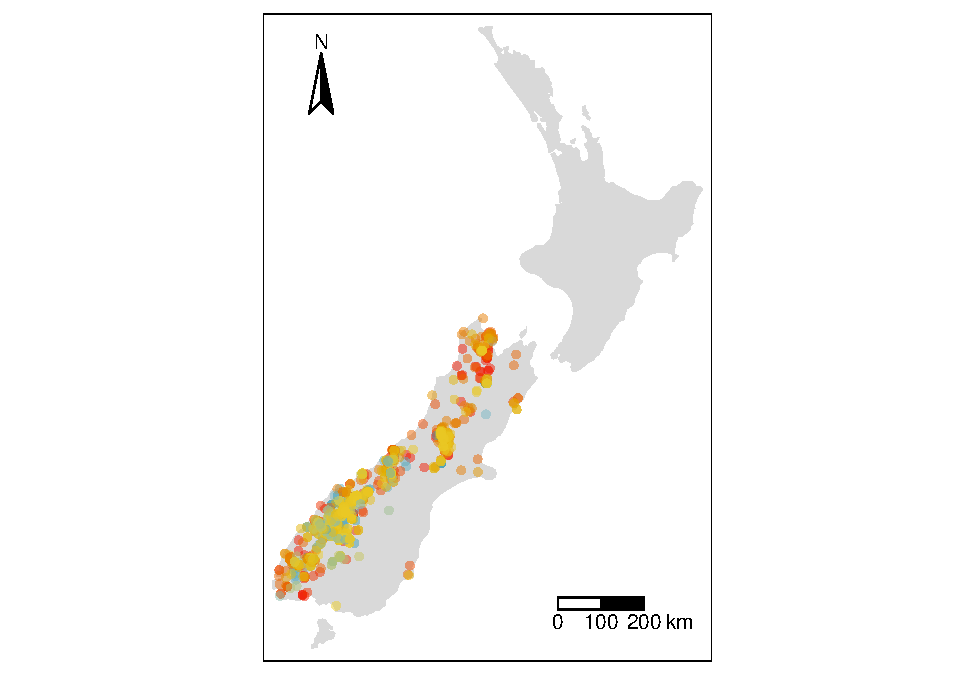
\includegraphics{kea_PVA_manuscript_files/figure-latex/Kea_map-1.pdf}
\caption{Kea sightings recorded since 1995 in the South Island of New
Zealand (data taken from \citet{Gbif2020}). Warmer colours indicate more
recent sightings}
\end{figure}

\hypertarget{model-structure}{%
\subsection{Model Structure}\label{model-structure}}

We implemented a stochastic simulation model incorporating three stage
classes to explore the effects of interactions between predation and HM
on kea population dynamics. The three stage classes were juveniles (0-1
year), sub-adults (1-3 years), and adults (3+ years). These stage
classes were selected to match significant changes in behaviour,
mortality risk, and breeding ability in the life history of the species.
The model represented the transition between each stage class, breeding,
and mortality (Figure 2). Mortality rates aggregated background,
predation mortality, and HM, with the level of predation and
human-induced mortality varied depending on the scenario being explored.

Only females were represented in the model as the kea's monogamous
reproductive status indicates that unpaired males rarely contribute to
population growth \citep{bond1991, ferson1995}. Furthermore, previous
research suggests there is a male sex-bias in wild populations, meaning
that females are more likely to form pair-bonds than males
\citep{bond1991, bond1992}. The demographic parameters in the model
varied stochastically through time but were perfectly correlated;
although this correlation in vital rates is unlikely, it is a more
conservative approach to assessing the population's viability than
treating each rate as independent \citep{ellner2002, ferson1995}. As the
model represents national mean population abundances and demographic
rates, and kea are endemic to New Zealand, we assumed a closed
population.

The model was constructed in R v3.6.2 \citep{R2020}, using the deSolve
package v1.27.1 \citep{soetaert2010}. The model ran for 250 timesteps
(each timestep representing one year). This period was chosen as it was
sufficient to detect demographic trends in long-lived species.

\begin{figure}
\centering
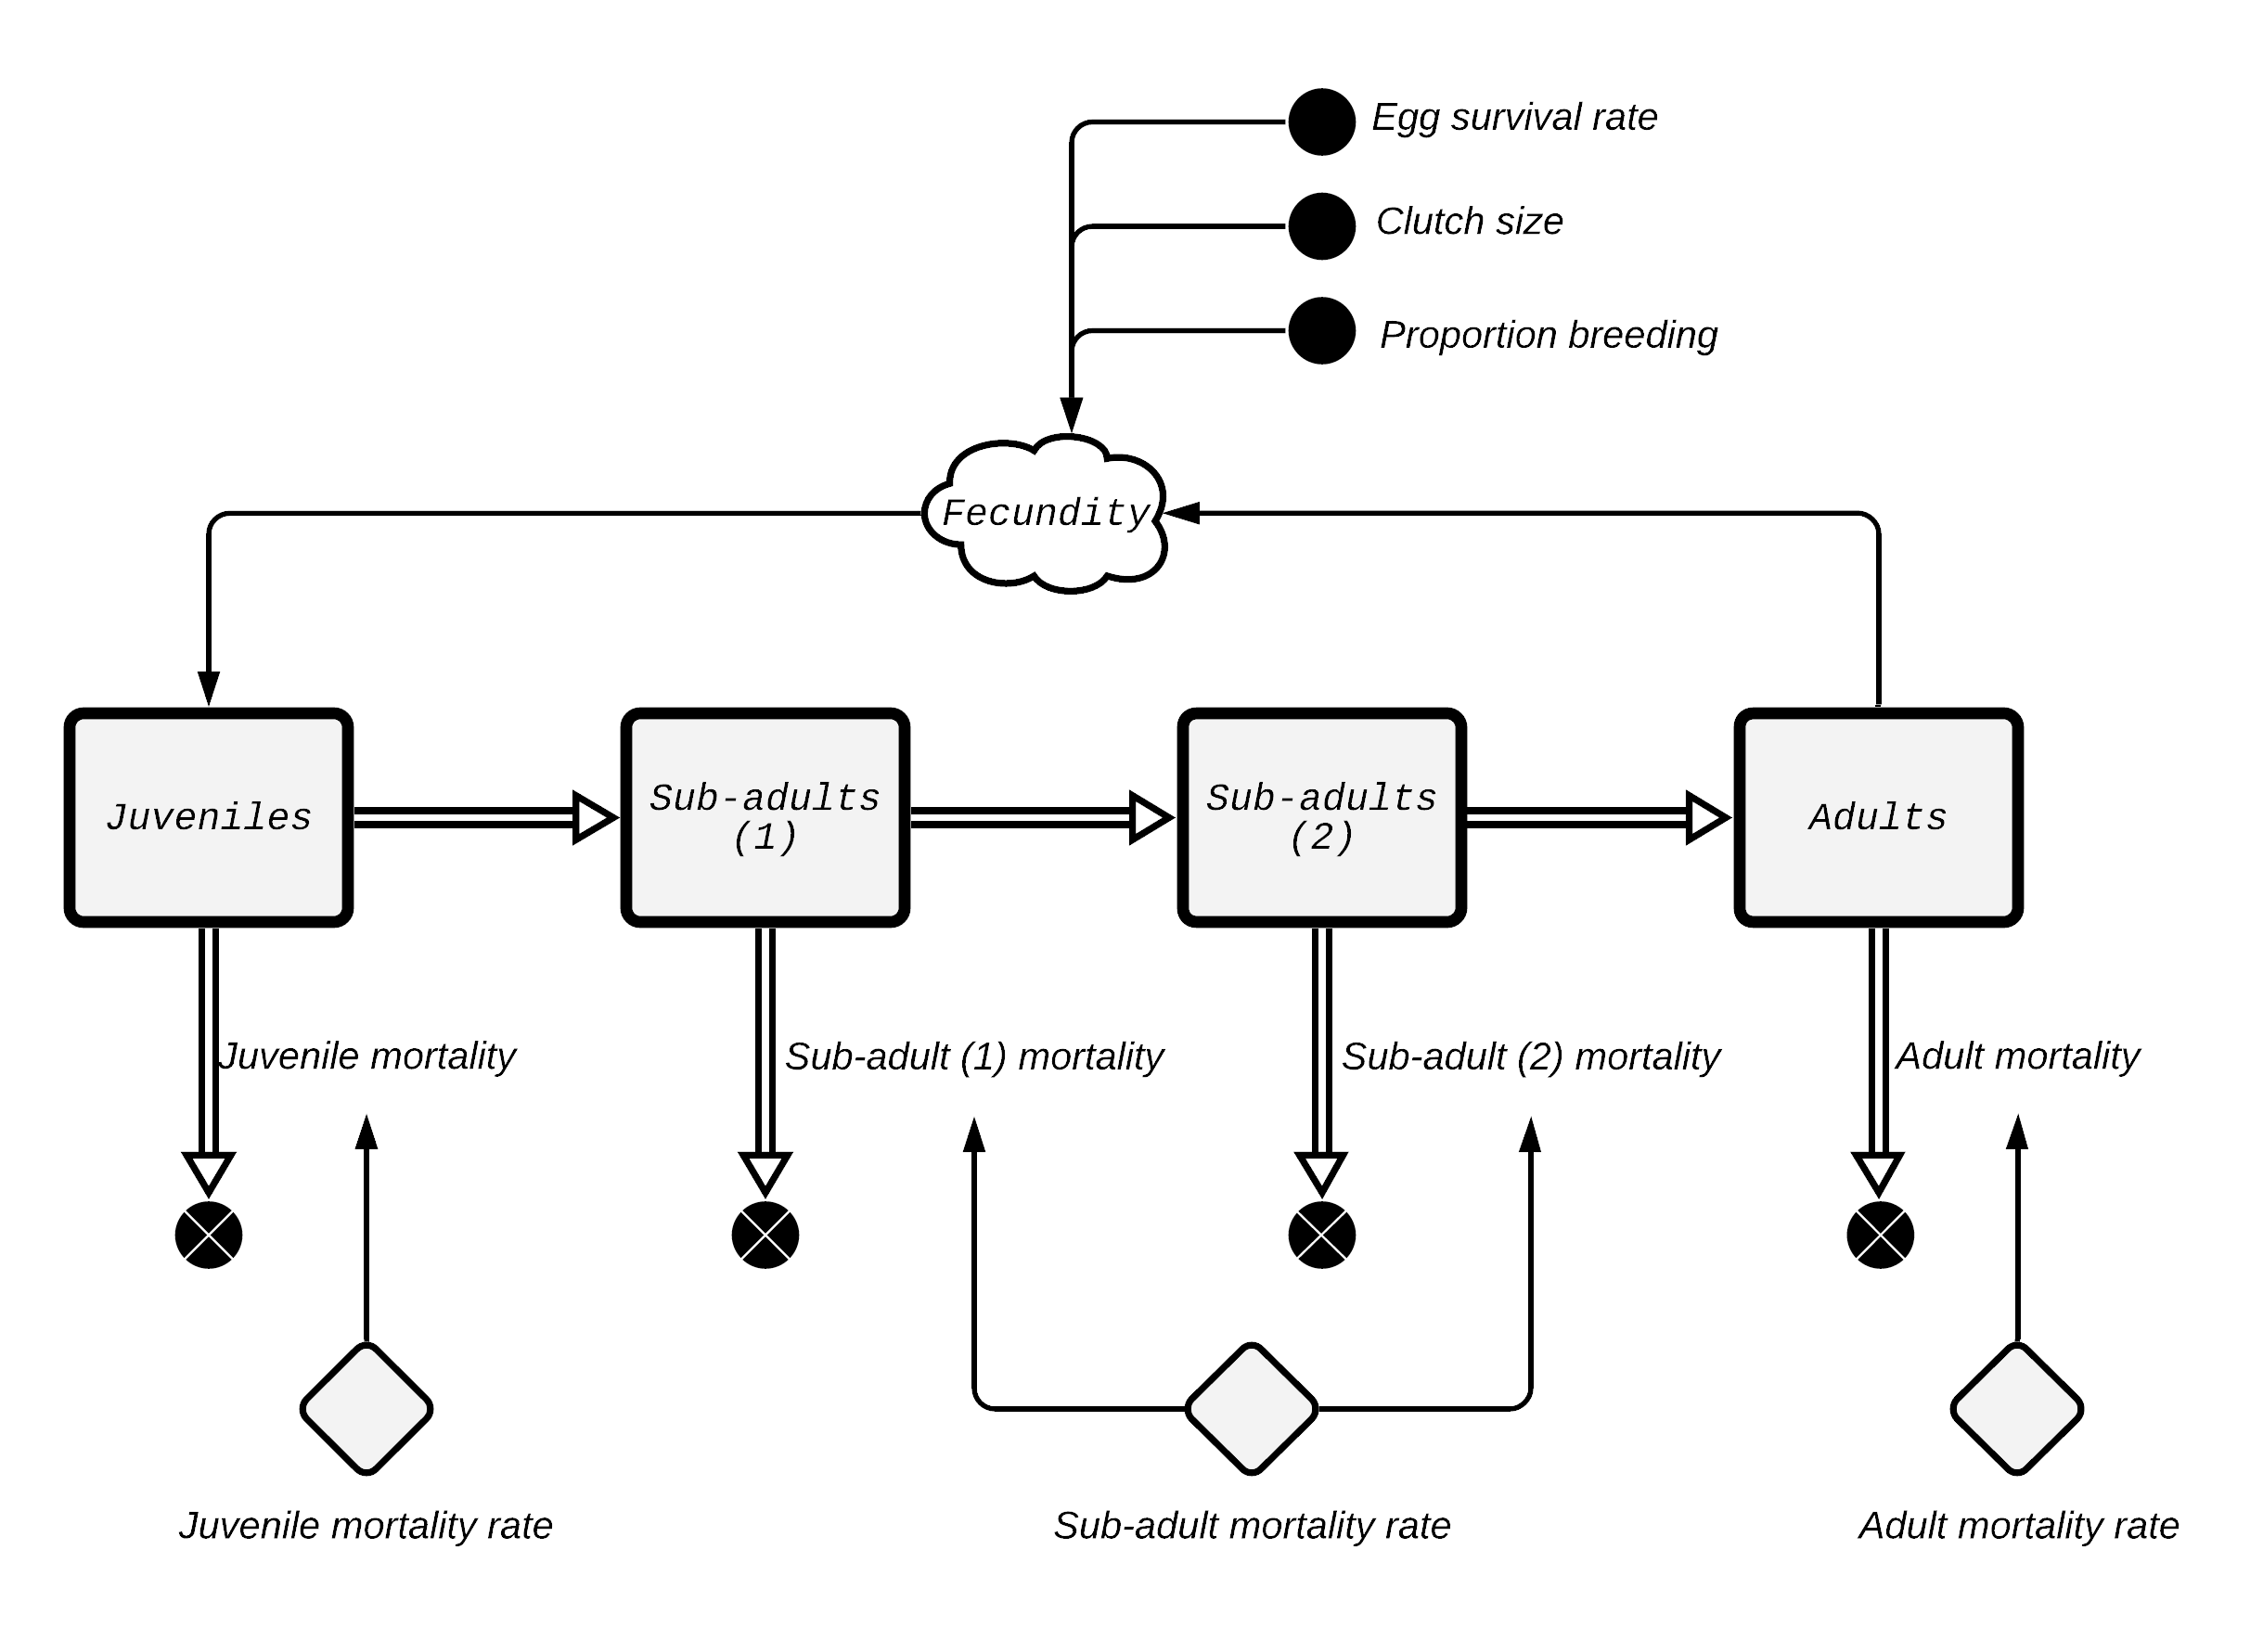
\includegraphics{Figures/Kea_model.png}
\caption{Overview of the kea population model. Rectangular boxes denote
the population stocks for each stage class, note to denote that kea
remain as sub-adults for two timesteps in the model there are two
sub-adult stocks. The double-lined arrows represent the flow of
individuals. The single-lined arrows represent connections between model
parameters. The grey diamonds denote variable rate factors, in this case
mortality rates.}
\end{figure}

\hypertarget{model-parameters}{%
\subsection{Model parameters}\label{model-parameters}}

\hypertarget{population-parameters}{%
\subsubsection{Population parameters}\label{population-parameters}}

Initial population size of 500 female kea was based on the lowest
published estimate \citep{pullar1996}. We used the lowest value because
there is considerable uncertainty in population estimates
\citep{orrWalker2009}, and we wanted to present a conservative rather
than optimistic estimate of extinction risk. To ensure that this choice
did not overly alter the results of the model the initial population
size was included as a parameter in the sensitivity analysis (see Model
execution and analysis section). We assumed an equal division of
individuals (i.e.~125 individuals within each stock) for the initial
timestep.

\hypertarget{reproduction}{%
\subsubsection{Reproduction}\label{reproduction}}

Kea have a mostly monogamous breeding system \citep{bond1991}, and begin
breeding from three years of age \citep{jackson1963}. To simulate this
behaviour only adult birds (over three years of age) bred in our model.
Fecundity was defined as the product of the number of adult females,
clutch size, and egg survival. The proportion of breeding adults was set
at 0.6 as not all females breed successfully every year
\citep{bond1991}. Clutch size for kea was generated using a bounded
Poisson distribution with a rate (\(\lambda\)) of 1.5 and with minimum
and maximum values of one and eight respectively. This value was
selected to generate clutch sizes similar to those observed in kea,
between 1-5, taking into account that only approximately half the chicks
would be female \citep{bond1992}.

\hypertarget{mortality}{%
\subsubsection{Mortality}\label{mortality}}

Mortality rates varied across the three stage classes. Mortality rates
were composed of predation, HM, and background mortality. Predation and
background mortality rates were based on the data collected by
\citet{seal1991} (Table 1). In addition, approximately every four years
a beech mast occurs \citep{ogden1996}, triggering irruptions of
mammalian predators that predate kea, leading to an increase in
predation mortality
\citep[\href{mailto:2001@elliott1996}{\nolinkurl{2001@elliott1996}};][]{choquenot2006}.
This masting dynamic was accounted for by adding a mast event with a
0.25 probability of occurring each time step. No temporal structure in
the pattern of masting was assumed, meaning that masts could occur in
successive years. To simulate the impact of a mammalian predator
population spike resulting from a mast the predation rate for all stage
classes increased by 0.1 during a mast time step. Stochasticity was
added to the baseline mortality rates by multiplying them by values
drawn from a random uniform distribution with values 10\% above and
below the baseline rate.

\begin{longtable}[]{@{}rcccc@{}}
\caption{Initial number of individuals in each stage class and predation
rates used in the PVA model. \emph{N} is the initial number of
individuals. Rates are all expressed as probability per
timestep/year.}\tabularnewline
\toprule
Stage class & \emph{N} & Current/baseline mortality & Low predation &
High predation\tabularnewline
\midrule
\endfirsthead
\toprule
Stage class & \emph{N} & Current/baseline mortality & Low predation &
High predation\tabularnewline
\midrule
\endhead
Egg & - & 0.4 & 0.2 & 0.8\tabularnewline
Juvenile & 125 & 0.2 & 0.1 & 0.4\tabularnewline
Sub-adult & 250 & 0.05 & 0.025 & 0.2\tabularnewline
Adult & 125 & 0.1 & 0.05 & 0.3\tabularnewline
\bottomrule
\end{longtable}

Department of Conservation's database was used to determine how many kea
deaths could be attributed to HM. We considered intentional causes
(e.g.~shooting, trapping) and accidental causes (e.g.~vehicle strike) as
HM. We assumed HM rates were the same across all stage-classes, although
no HM was assigned to eggs, as kea nests are cryptic and there is
minimal chance of people interacting with them. To represent potential
changes in HM due to human population change over time we evaluated
three potential population scenarios: 1) No HM (baseline); 2) HM at a
constant rate of 0.015 (matching the currently observed HM rate); and 3)
a linear increase in HM. The linear rate of increase was set as 0.0003
per time step (i.e.~an increment of 2\% of the currently observed HM
rate per time step). This rate was selected to match the approximate 2\%
national human population population growth rate, assuming a one to one
relationship between population size and HM.

Linear growth was calculated as: \begin{equation}
  M_{t+1} = M_{t} + C
\end{equation}

Where \(M\) is mortality and \(C\) is the rate of change in the
population.

\hypertarget{model-execution-and-analysis}{%
\subsection{Model execution and
analysis}\label{model-execution-and-analysis}}

Each scenario was evaluated by running 1000 simulations of 250 timesteps
each (unless the population reached zero before this time). We used a
critical population size as a `quasi-extinction' threshold
\citep{morris2002}, as this is often used to set conservation policy
\citep{mace1991}. We defined the quasi-extinction threshold as a
population of 50 individuals \citep{holmes2007, otway2004}. Time until
extinction was determined by calculating the first year in which the
quasi-extinction threshold was passed. The overall extinction risk was
estimated as the proportion of replicates for each scenario which
experienced a quasi-extinction (i.e.~\(N < 50\)).

Mean population growth rates for each scenario were determined using the
mean geometric growth: \begin{equation}
  \lambda_g = (\frac{N_t}{N_0})^{\frac{1}{t}}
\end{equation}

Where \(\lambda_g\) is the growth rate; \(N_t\) is the number of kea at
time \(t\); and \(N_0\) is the number of kea at time zero. To check
whether any observed differences between scenarios were statistically
notable we used the Cohen D effect size metric, which measures the size
of an experimental effect (see \citet{nakagawa2007} for additional
details on effect size statistics).

We also conducted a local univariate sensitivity analysis for initial
population size, clutch size and the proportion of breeding adults,
which were determined to be demographic values with a high level of
uncertainty. The sensitivity analysis was run using current/baseline
predation rates and no HM. Each parameter was individually varied by
\(\pm 10 \%\) and \(\pm 25 \%\) of their baseline value and the model
run for 250 timesteps for 1000 repeats with each value. As the clutch
size was drawn from a Poisson distribution the \(\lambda\) of this
distribution was altered. The parameter sensitivities were determined
using the index described by \citet{hamby1994}. \begin{equation}
  S_{y,x} = \frac{(\frac{\Delta y}{y_b})}{(\frac{\Delta x}{x_b})}
\end{equation}

Where \(S_{y,x}\) is the sensitivity of the output variable \(y\) to a
change in the input variable \(x\). \(\Delta y\) is the change in output
variable \(y\), \(y_b\) is the baseline output. \(\Delta x\) is the
change in input variable \(x\), \(x_b\) is the baseline input. The final
population size aggregated across all stage classes was used as the
output variable of interest and a parameter was considered to be
`sensitive' if the index resulted in a value \textgreater{} 1.

\hypertarget{results}{%
\section{Results}\label{results}}

\hypertarget{predation-management}{%
\subsection{Predation management}\label{predation-management}}

Of the 3000 runs with no additional HM, 1029 (34.3\%) resulted in
extinction events (i.e.~population dropping below 50 individuals). The
high predation scenario showed a 100\% extinction rate (i.e.~1000
extinction events) with a mean time until extinction of 8 \(\pm\) 0.7
years (mean \(\pm\) 1 SD). To explore whether the high rate of
extinction seen in the high predation scenario was influenced by
population size we run the model again with an initial population
\(10 \%\) and \(25 \%\) higher. Each initial population setting was run
for a maximum of 250 timesteps for 1000 repeats. An increase to the
initial population size did not have any notable effect on the high
predation scenario results, with both initial population abundances
experiencing a 100\% extinction rate and a time until extinction of less
than 10 years.Under the baseline predation scenario 11 of the 1000
simulations ended in extinction, with a mean time until extinction of
106 \(\pm\) 73.3 years. Interestingly, the low predation scenario runs
resulted in 18 extinctions, slightly higher than the baseline scenario,
although this small difference is likely due to the stochastic nature of
the model, and as stated below abundances tended to be higher in the low
predation scenario.

All three predation scenarios showed an initial burn-in in population,
representing initial transient dynamics, followed by a continuing period
of relatively unchanging population numbers (Figure 3). The high
predation scenario clearly had a higher mortality rate than replacement
rate, resulting in rapid extinction. Under baseline/current predation
levels there was an initial decrease in the number of individuals,
quickly reaching a stable level of approximately 350 females. Under low
predation levels, the rate of replacement outstripped mortality
initially, resulting in a period of population growth followed by a
stable period with a population of approximately 500 individuals. These
trends were mirrored in the mean population sizes of each predation
scenario with high predation having the lowest population (6 \(\pm\)
0.4), being a lot lower (Cohen D = 19.7) than the baseline/current
predation scenario (335 \(\pm\) 24), which was considerably lower (Cohen
D = 5.4) than the low predation scenario (527 \(\pm\) 45).

The mean growth rates for the three predation scenarios showed the same
trend as discussed above. The high predation scenario showed the lowest
growth rate (0.072 \(\pm\) 0.008), which was far lower (Cohen D = 5.5)
than that under the baseline/current predation scenario (0.992 \(\pm\)
0.001). There was only a notable difference (Cohen D = 0.5) between the
baseline/current predation scenario growth rate, and the low predation
scenario growth rate (0.984 \(\pm\) 0.098), though this was likely
reduced by the long period of stable population for each scenario.

\begin{figure}
\centering
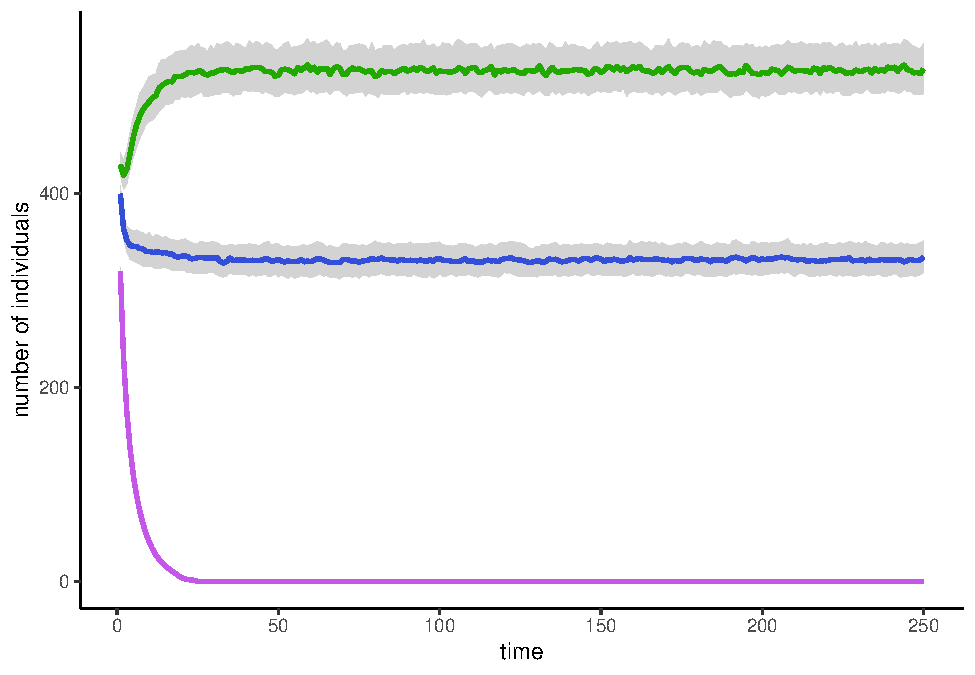
\includegraphics{kea_PVA_manuscript_files/figure-latex/Population timeseries figure-1.pdf}
\caption{Change in the median number of individuals through time for
each of the predation scenarios. The green line is the low predation
scenario; blue line is the baseline/current predation scenario; and the
violet line is the high predation scenario. The gray bands represent the
33\textsuperscript{rd} to 66\textsuperscript{th} quantile band}
\end{figure}

\hypertarget{human-induced-mortality}{%
\subsection{Human-induced mortality}\label{human-induced-mortality}}

Due to the large difference in values for the high predation scenario
compared to the baseline/current and low predation scenarios it was
removed from the analysis of HM to avoid any trends being obscured.

There were only minor differences in the overall extinction rate across
the three HM scenarios for either baseline/current or low predation
(Table 2). Notably, the no additional HM scenarios had the highest rates
of extinction (1.1\% of baseline/current predation runs and 1.8\% of low
predation runs), likely due to the stochastic nature of the model.
Again, there were only small differences in the mean time until
extinction of each scenario, although the rankings for the different HM
scenarios differed from that of predation rate.

\begin{longtable}[]{@{}rcccc@{}}
\caption{Percentage of total runs ending in quasi-extinction (i.e.~fewer
than 50 individuals), mean time for an extinction event to occur, and
the mean number of females for each human-induced mortality scenario
under baseline/current and low predation levels.}\tabularnewline
\toprule
\begin{minipage}[b]{0.16\columnwidth}\raggedleft
Predation level\strut
\end{minipage} & \begin{minipage}[b]{0.17\columnwidth}\centering
Human-induced mortality scenario\strut
\end{minipage} & \begin{minipage}[b]{0.17\columnwidth}\centering
Percentage of runs ending in extinction\strut
\end{minipage} & \begin{minipage}[b]{0.17\columnwidth}\centering
Mean time-steps until extinction (\(\pm\) standard deviation)\strut
\end{minipage} & \begin{minipage}[b]{0.17\columnwidth}\centering
Mean population size (\(\pm\) standard deviation)\strut
\end{minipage}\tabularnewline
\midrule
\endfirsthead
\toprule
\begin{minipage}[b]{0.16\columnwidth}\raggedleft
Predation level\strut
\end{minipage} & \begin{minipage}[b]{0.17\columnwidth}\centering
Human-induced mortality scenario\strut
\end{minipage} & \begin{minipage}[b]{0.17\columnwidth}\centering
Percentage of runs ending in extinction\strut
\end{minipage} & \begin{minipage}[b]{0.17\columnwidth}\centering
Mean time-steps until extinction (\(\pm\) standard deviation)\strut
\end{minipage} & \begin{minipage}[b]{0.17\columnwidth}\centering
Mean population size (\(\pm\) standard deviation)\strut
\end{minipage}\tabularnewline
\midrule
\endhead
\begin{minipage}[t]{0.16\columnwidth}\raggedleft
Baseline\strut
\end{minipage} & \begin{minipage}[t]{0.17\columnwidth}\centering
None\strut
\end{minipage} & \begin{minipage}[t]{0.17\columnwidth}\centering
1.1\strut
\end{minipage} & \begin{minipage}[t]{0.17\columnwidth}\centering
106 \(\pm\) 73\strut
\end{minipage} & \begin{minipage}[t]{0.17\columnwidth}\centering
335 \(\pm\) 24\strut
\end{minipage}\tabularnewline
\begin{minipage}[t]{0.16\columnwidth}\raggedleft
Baseline\strut
\end{minipage} & \begin{minipage}[t]{0.17\columnwidth}\centering
Static\strut
\end{minipage} & \begin{minipage}[t]{0.17\columnwidth}\centering
0.8\strut
\end{minipage} & \begin{minipage}[t]{0.17\columnwidth}\centering
146 \(\pm\) 92\strut
\end{minipage} & \begin{minipage}[t]{0.17\columnwidth}\centering
297 \(\pm\) 20\strut
\end{minipage}\tabularnewline
\begin{minipage}[t]{0.16\columnwidth}\raggedleft
Baseline\strut
\end{minipage} & \begin{minipage}[t]{0.17\columnwidth}\centering
Linear\strut
\end{minipage} & \begin{minipage}[t]{0.17\columnwidth}\centering
0.4\strut
\end{minipage} & \begin{minipage}[t]{0.17\columnwidth}\centering
219 \(\pm\) 61\strut
\end{minipage} & \begin{minipage}[t]{0.17\columnwidth}\centering
211 \(\pm\) 9\strut
\end{minipage}\tabularnewline
\begin{minipage}[t]{0.16\columnwidth}\raggedleft
Low\strut
\end{minipage} & \begin{minipage}[t]{0.17\columnwidth}\centering
None\strut
\end{minipage} & \begin{minipage}[t]{0.17\columnwidth}\centering
1.8\strut
\end{minipage} & \begin{minipage}[t]{0.17\columnwidth}\centering
119 \(\pm\) 75\strut
\end{minipage} & \begin{minipage}[t]{0.17\columnwidth}\centering
527 \(\pm\) 45\strut
\end{minipage}\tabularnewline
\begin{minipage}[t]{0.16\columnwidth}\raggedleft
Low\strut
\end{minipage} & \begin{minipage}[t]{0.17\columnwidth}\centering
Static\strut
\end{minipage} & \begin{minipage}[t]{0.17\columnwidth}\centering
0.7\strut
\end{minipage} & \begin{minipage}[t]{0.17\columnwidth}\centering
160 \(\pm\) 52\strut
\end{minipage} & \begin{minipage}[t]{0.17\columnwidth}\centering
487 \(\pm\) 19\strut
\end{minipage}\tabularnewline
\begin{minipage}[t]{0.16\columnwidth}\raggedleft
Low\strut
\end{minipage} & \begin{minipage}[t]{0.17\columnwidth}\centering
Linear\strut
\end{minipage} & \begin{minipage}[t]{0.17\columnwidth}\centering
1.4\strut
\end{minipage} & \begin{minipage}[t]{0.17\columnwidth}\centering
128 \(\pm\) 74\strut
\end{minipage} & \begin{minipage}[t]{0.17\columnwidth}\centering
393 \(\pm\) 27\strut
\end{minipage}\tabularnewline
\bottomrule
\end{longtable}

The general impact of the different HM scenarios on the number of
individuals in the population was the same for baseline/current and low
predation levels (Figure 4). Linearly increasing HM resulted in far
lower (Cohen D \textgreater{} 3.0) population sizes for both
baseline/current (211 \(\pm\) 9) and low (393 \(\pm\) 27) predation
levels than either static or no HM scenarios. Linearly increasing HM
also produced a declining population trend, resulting in larger
differences with the other scenarios as model runs progressed (Figure
4). Static and no HM scenarios produced similar outcomes, though static
HM had consistently lower population sizes for both baseline/current
(297 \(\pm\) 20 compared to 335 \(\pm\) 24 for no HM) and low (487
\(\pm\) 19 compared to 527 \(\pm\) 45 for no HM) predation levels, with
these differences having a large effect size (Cohen D = 2 and Cohen D =
1 for baseline and low predation level scenarios, respectively). The
trend in mean population size is reflected in the mean growth rate
produced by each scenario (Figure 6.).

\begin{figure}
\centering
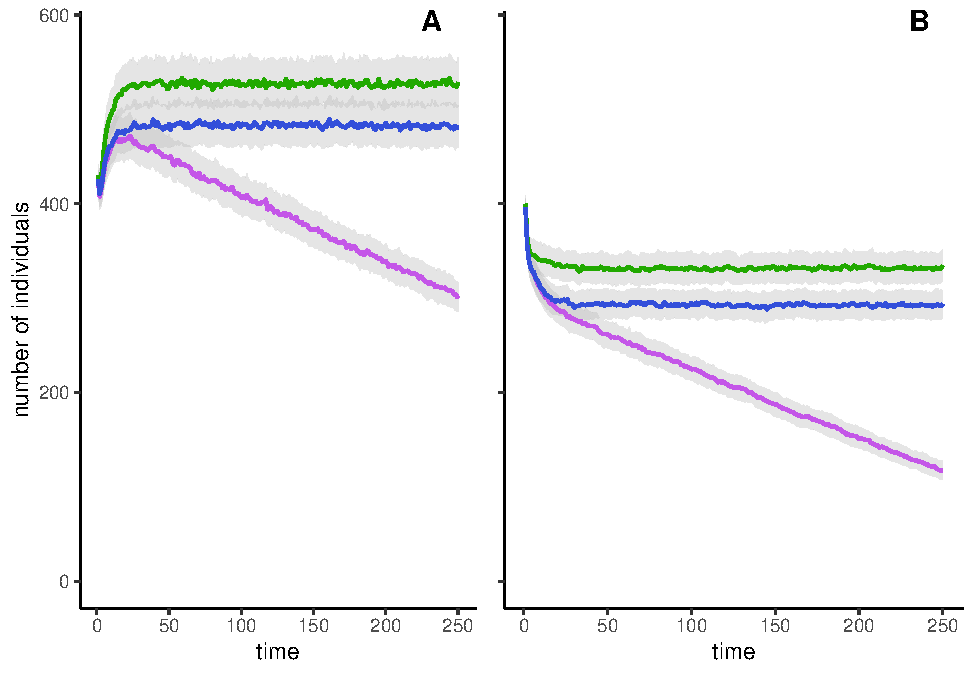
\includegraphics{kea_PVA_manuscript_files/figure-latex/Population timeseries for HIM figure-1.pdf}
\caption{Change in the median number of individuals (pooled across all
stage classes) through time for each of the HM scenarios under low (A)
and baseline/current (B) predation levels. The blue lines are the static
HM scenarios; violet lines are the linearly increasing HM scenarios; and
the green lines are the no HM scenarios. The gray bands represent the
33\textsuperscript{rd} to 66\textsuperscript{th} quantile band}
\end{figure}

\begin{figure}
\centering
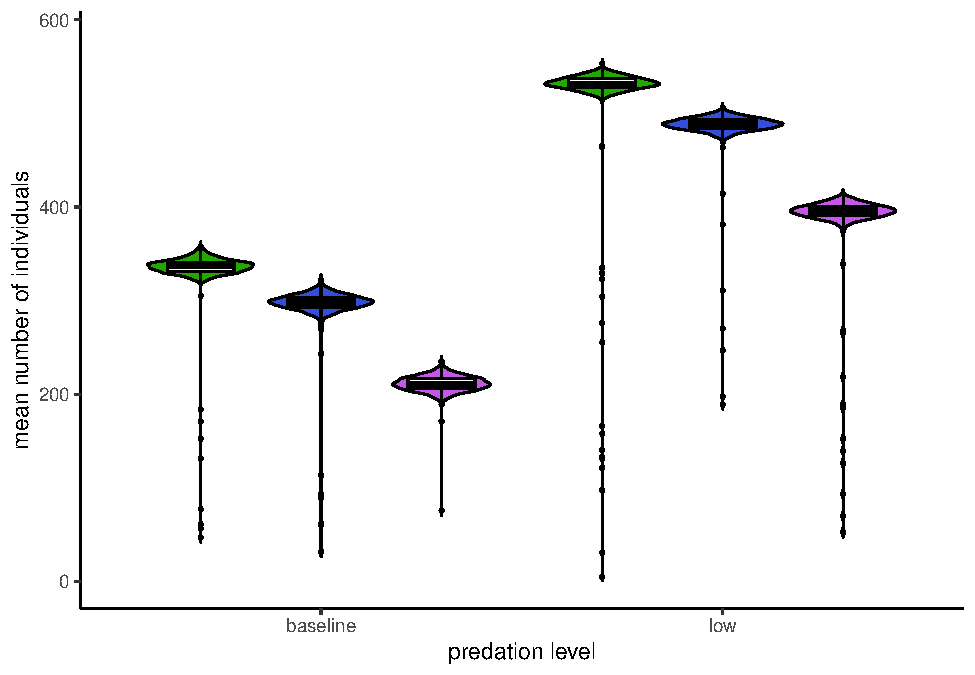
\includegraphics{kea_PVA_manuscript_files/figure-latex/Average population for HIM violin plot-1.pdf}
\caption{The mean number of individuals (pooled across all stage
classes) after 250 years for each of the 1000 simulations of each of the
HM scenarios under low and baseline/current predation levels. The green
distributions are the no HM scenario; the center blue distributions are
the static HM scenario; and the violet distributions are the linearly
increasing HM scenario.}
\end{figure}

\begin{figure}
\centering
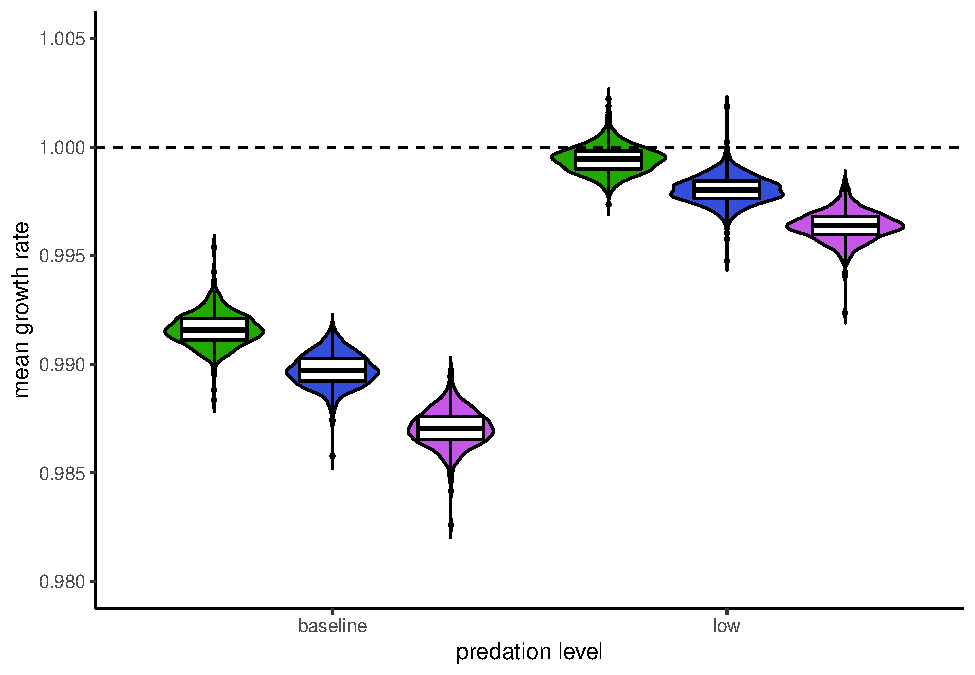
\includegraphics{kea_PVA_manuscript_files/figure-latex/Average growth rate for HIM violin plot-1.pdf}
\caption{The mean growth rate for each of the 1000 runs for each of the
HM scenarios under low and baseline/current predation levels. The green
distributions are the no HM scenario; the blue distributions are the
static HM scenario; and the violet distributions are the linearly
increasing HM scenario.}
\end{figure}

\hypertarget{sensitivity-analysis}{%
\subsection{Sensitivity Analysis}\label{sensitivity-analysis}}

The model was not sensitive to any of the three parameters tested
(initial population size, clutch size, or proportion of breeding
females) at either the \(\pm 10 \%\) or \(\pm 25 \%\) (Table 3). This
suggests that the model outcomes were robust to uncertainty in
estimating these parameters.

\begin{longtable}[]{@{}rcccc@{}}
\caption{Sensitivity values calculated for each of the three tested
parameters at each of the four percentage change values. Higher values
indicate that the model is more sensitive to those changes, with values
greater than one suggesting the model is disproportionately sensitive to
that change.}\tabularnewline
\toprule
Parameter & Plus 25\% & Plus 10\% & Minus 10\% & Minus
25\%\tabularnewline
\midrule
\endfirsthead
\toprule
Parameter & Plus 25\% & Plus 10\% & Minus 10\% & Minus
25\%\tabularnewline
\midrule
\endhead
Initial population & 0.08 & 0.01 & 0.23 & 0.04\tabularnewline
Clutch size & 0.28 & 0.15 & 0.12 & 0.16\tabularnewline
Proportion breeding & 0.18 & 0.17 & 0.28 & 0.29\tabularnewline
\bottomrule
\end{longtable}

\hypertarget{discussion}{%
\section{Discussion}\label{discussion}}

Our model outcomes clearly demonstrate that changes in either the level
of mammalian predation or the HM rate may have dramatic effects on the
population dynamics of kea. An increase in the rate of predation had the
most substantial impact of the population, with all high predation
simulations quickly ending in extinction (Figure 3), with this outcome
being insensitive to changes in initial population size. This result
highlights the importance of ongoing predator management for the
survival of kea. While a decrease in the predation level to below the
current managed rate, such as may be achieved under the predator free
2050 project \citep{Russell2015}, would see an increase in kea numbers,
current management appears sufficient to maintain a stable population
with a relatively low likelihood of extinction. \citet{kemp2018} came to
a similar conclusion when evaluating kea nest survival after the
application of aerial sodium fluoroacetate (``Compound 1080''), showing
both a decline in nest survival in areas without pest management and a
substantial increase in nest survival following predator management.
Furthermore, the management of mammalian predators is the most
significant factor in determining the long term survival for a number of
other New Zealand bird species (e.g.~mohua (\emph{Mohoua ochrocephala})
\citep{elliott1996}, whio (\emph{Hymenolaimus malacorhynchos})
\citep{simpkins2015}, brown kiwi (\emph{Apteryx mantelli})
\citep{Basse1999}, and others see \citet{Fea2020}). Our study adds to
the consensus that mammalian predator management is a fundamental factor
in the conservation process for New Zealand.

While predation had the largest impact on kea population dynamics,
increased HM also had a substantial effect on the kea population. At its
current rate, HM had only a small negative impact on population size
(and no noticeable impact on extinction risk). While any reduction in
population size does decrease the resilience of the population making
more susceptible to factors such as habitat loss or climate change
\citep{Keith2008}, the level of change observed under current levels of
HM is likely too low to concern conservation managers. However, it is
unlikely that HM will remain at its current level, if unmanaged, given
the growth in the resident human population of New Zealand, tourism
rates, and the correlation between human population and HWC events
\citep{Kretser2008}. As HM rates increase over time they have an
increasingly large negative effect on the kea population. Given the
current low impact of HM coupled with its likely growth over time, it
would be best for HM sources (e.g.~vehicle collisions) to become
actively managed as soon as feasible. This intervention would allow time
for management practices to improve and become embedded before HM
reaches a level of significant concern for the kea population.

The model outcomes should be viewed qualitatively, as opposed to
quantitatively, as there is considerable uncertainty in a some
parameters \citep{coulson2001}, although the model does appear robust to
this uncertainty. First, the base HM are likely higher than were
included in the model, because many HM events may not be reported or
detected, although this discrepancy is difficult to quantify. Second, we
did not include indirect or secondary HM events as these are difficult
to assign as being human-induced events. Of particular concern is the
changes in mortality rates that may occur due to kea ingesting human
food, such as chocolate, which may have long-term detrimental health
effects \citep{gartrell2007}. However, access to additional resources in
times of scarcity may also decrease mortality rates during some periods,
and even potentially allow for a larger sustainable population. Third,
in implementing and parameterising the model (e.g.~correlation of
demographic parameters) we chose the most conservative approach.
Therefore, it is likely that our population estimates may be slightly
small; however, as we have not accounted for additional stressors, such
as climate change, this overly cautious approach is likely justifiable.
This uncertainty in parameter values, and thus in the precise values of
the model outcomes, furthers our recommendation that management for HM
be taken before it becomes a substantial threat to the population,
rather than waiting for predictions of HM to become a concern.

\hypertarget{acknowledgements}{%
\section{Acknowledgements}\label{acknowledgements}}

We thank Finnbar Lee and Andre Bellve for their help in improving the
manuscript.

\hypertarget{data-accessibility}{%
\section{Data accessibility}\label{data-accessibility}}

All the data used as well as a reproducible notebook containing the
scripts to recreate this paper, including all figures, are available at
\url{https://github.com/csim063/kea_human_wildlife_conflict}.

\newpage
\singlespacing 
\renewcommand\refname{References}
\bibliography{References/master.bib}
\end{document}